\begin{problem}{Tengdur Listi}{Inn}{Út}{~}{~}

	Gagnaskipan sem oft er notað í Tölvunarfræði kallast Tengdur listi. Hann er notaður til að geyma runu af stökum (líkt og fylki), en að framkvæma mismunandi aðgerðir (eins og að bæta við staki, fjarlægja stak, eða ná í stak á ákveðnum stað) getur verið bæði hægara eða hraðara en á venjulegu fylki sem inniheldur sömu stök. Tengdur listi er ekki einungis gagnlegur einn og sér, heldur er hann líka grunnurinn að mörgum flóknari gagnaskipan.

	Tengdur listi samanstendur af svokölluðum hnútum. Hver hnútur geymir ákveðið stak í listanum, og bendir svo á næsta hnút. Síðasti hnúturinn í listanum geymir síðasta stakið í listanum, og bendir svo ekki neitt, eða hefur svo kallaðan "`\textit{NULL}"' bendi.

	\begin{figure}[h]
		\centering
		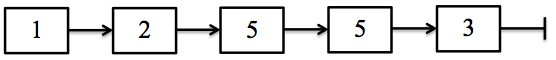
\includegraphics[scale=0.4]{../TengdurListi/linkedlist.png}
	\end{figure}

	Tökum sem dæmi tengdan lista með stökunum $5, 8, 5 \textrm{ og } 7$ í þeirri röð. Þá er einn hnútur fyrir hvert stak, og hver hnútur bendir á þann næsta. Síðasti hnúturinn hefur svo "`\textit{NULL}"' bendi. Tengdi listinn fyrir stökin að ofan má tákna á eftirfarandi hátt:

	\begin{center}
		\texttt{[5]->[8]->[5]->[7]->NULL}
	\end{center}

	Ein aðgerð sem oft þarf að gera á tengan lista er að snúa honum við. Til dæmis, ef við snúum listanum að ofan við, þá fáum við eftirfarandi tengdan lista:

	\begin{center}
		\texttt{[7]->[5]->[8]->[5]->NULL}
	\end{center}

	Þú átt að lesa inn tengdan lista sem er táknaður á þessu formi, snúa honum við, og skrifa hann út á sama formi.

	\Input

		Á fyrstu línu er heiltalan $1 \leq T \leq 100$, sem táknar fjölda tengdra lista til að snúa við. Svo fylgja $T$ línur, þar sem hver lína er tengdur listi á forminu sem sýnt er að ofan. Gera má ráð fyrir að hver tengdur listi innihaldi að minnsta kosti eitt stak, og að hvert stak sé heiltala á bilinu 0 til 10000.

	\Output

		Fyrir hvern tengdan lista í inntakinu á að skrifa út eina línu sem inniheldur tengda listann þegar búið er að snúa honum við, líka á forminu sem sýnt er að ofan.

	\Examples

		\begin{example}
			\exmp{
5
[5]->[8]->[5]->[7]->NULL
[1]->[2]->[3]->NULL
[0]->[150]->[300]->NULL
[16]->[8]->[16]->NULL
[1337]->NULL
			}{
[7]->[5]->[8]->[5]->NULL
[3]->[2]->[1]->NULL
[300]->[150]->[0]->NULL
[16]->[8]->[16]->NULL
[1337]->NULL}%
		\end{example}

\end{problem}